\documentclass[a4paper]{article}

%% Language and font encodings
\usepackage[english]{babel}
\usepackage[utf8x]{inputenc}
% \usepackage[T1]{fontenc}
\usepackage{float}
\usepackage{url}

\usepackage{helvet}
\renewcommand{\familydefault}{\sfdefault}

%% Sets page size and margins
\usepackage[a4paper,top=3cm,bottom=2cm,left=3cm,right=3cm,marginparwidth=1.75cm]{geometry}

%% Useful packages
\usepackage{amsmath}
\usepackage{graphicx}
\usepackage[colorinlistoftodos]{todonotes}
\usepackage[colorlinks=true, allcolors=blue]{hyperref}


\usepackage{listings}
\lstset{basicstyle=\ttfamily,
  showstringspaces=false,
  commentstyle=\color{blue},
  keywordstyle=\color{black}
}

\title{Exercise 4: Training End-to-end driving networks}
\author{Michael Floßmann, Kshitij Sirohi, Hendrik Vloet}
\pagestyle{empty}
\begin{document}
\maketitle

\section{Introduction}
\subsection{Goals}
The main objective of this assignment was to get to know the rAIScar hardware
and apply the things learned in the previous exercises to port the ML algorithm
to the platform. This included:
\begin{itemize}
\item Finish unfinished tasks from the previous exercise sheet
\item Get familiar with the rAIScar hardware to collect the training data
  (collecting and converting data for the training infrastructure)
\end{itemize} 

\section{Training process}
TODO

\section{Leftover tasks from Exercise 3}

\subsection{Issues}
There were several issues to overcome which weren't completely solved in time.
One big issue was that the meaning of the braking information was quite cryptic
and after asking the original paper authors of \cite{imitation}, it turned out
that the braking and acceleration data was supposed to be fused into one
variable. After this was done, the networks trained properly, as can be seen in
the loss plots (figures \ref{fig:augmented_command_loss}.
\ref{fig:augmented_branched_loss}, \ref{fig:unaugmented_branched_loss}).

\begin{figure}[!htbp]
  \centering
  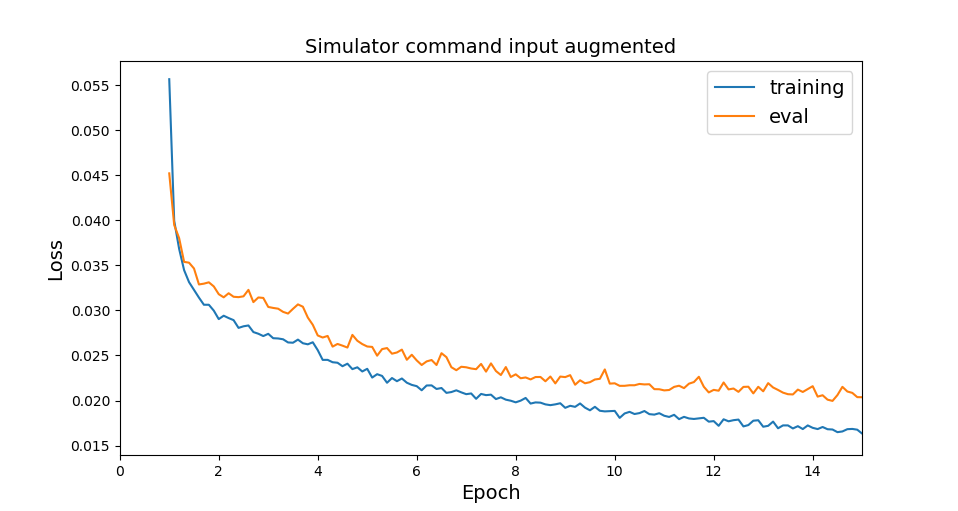
\includegraphics[width=0.95\textwidth]{figures/sim_command_input_aug_lossplot}
  \label{fig:augmented_command_loss}
  \caption{Simulation command input lossplot}
\end{figure}

\begin{figure}[!htbp]
  \centering
  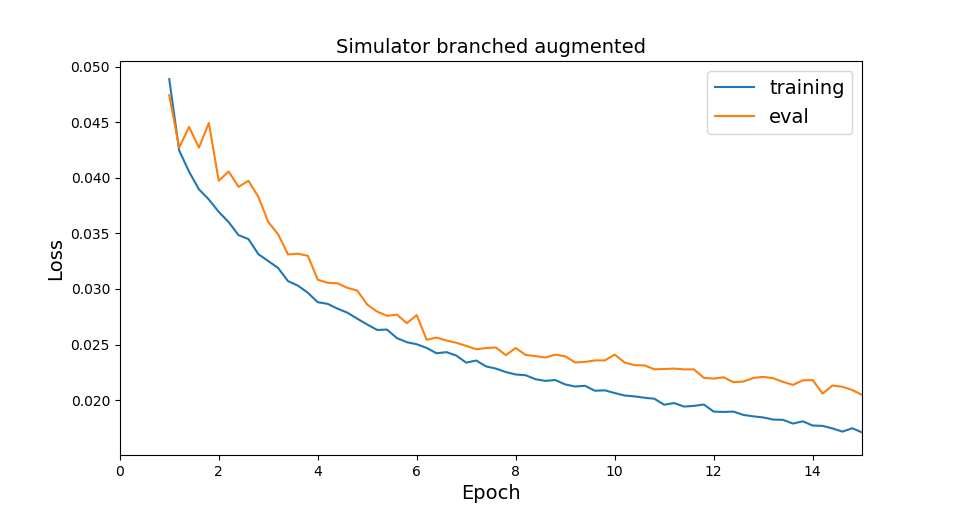
\includegraphics[width=0.95\textwidth]{figures/sim_branched_aug_lossplot}
  \label{fig:augmented_branched_loss}
  \caption{Simulation branched lossplot}
\end{figure}

\begin{figure}[!htbp]
  \centering
  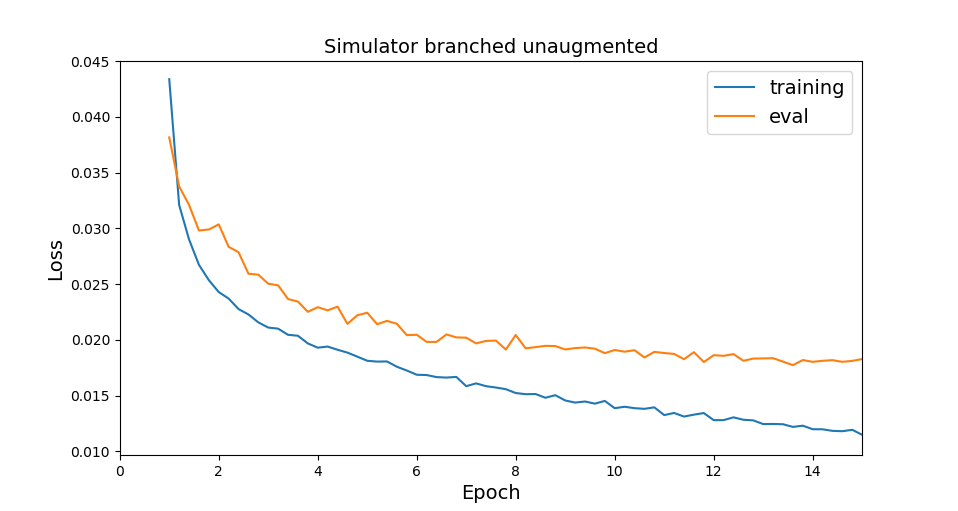
\includegraphics[width=0.95\textwidth]{figures/sim_branched_nonaug_lossplot}
  \label{fig:unaugmented_branched_loss}
  \caption{Simulation branched, unaugmented lossplot}
\end{figure}
	
\begin{thebibliography}{9}
\bibitem{imitation}
Codevilla, Felipe and Müller, Matthias and López, Antonio and Koltun, Vladlen
and Dosovitskiy, Alexey.
\textit{End-to-end Driving via Conditional Imitation Learning.}
ICRA 2018
\end{thebibliography}

\end{document}